\documentclass{standalone}
\usepackage{tikz}
\usepackage{ctex,siunitx}
\setCJKmainfont{Noto Serif CJK SC}
\usepackage{tkz-euclide}
\usepackage{amsmath}
\usetikzlibrary{patterns, calc}
\usetikzlibrary {decorations.pathmorphing, decorations.pathreplacing, decorations.shapes,}
\begin{document}
\small
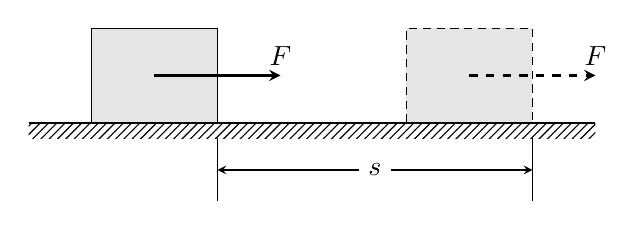
\begin{tikzpicture}[>=stealth,scale=.8]
  \fill [pattern = north east lines] (0,-.25) rectangle (9,0);
  \draw [fill=gray!20] (1,0) rectangle (3,1.5);
  \draw [densely dashed, fill=gray!20] (6,0) rectangle (8,1.5);
  \draw [semithick](0,0)--(9,0);
  \draw [thick,->] (2,1.5/2)--(4,1.5/2) node [above]{$F$};
  \draw [thick,dashed, ->] (7,1.5/2)--(9,1.5/2) node [above]{$F$};
  \draw [thin,<->](3,-0.75)--node [fill=white]{$s$}(8,-0.75);
  \draw [thin](3,-.25)--(3,-1.25);
  \draw [thin](8,-.25)--(8,-1.25);
\end{tikzpicture}
\end{document}